%%%%%%%%%%%%%%%%%%%%%%%%%%%%%%%%%%%%%%%%%
% FRI Data Science_report LaTeX Template
% Version 1.0 (28/1/2020)
% 
% Jure Demšar (jure.demsar@fri.uni-lj.si)
%
% Based on MicromouseSymp article template by:
% Mathias Legrand (legrand.mathias@gmail.com) 
% With extensive modifications by:
% Antonio Valente (antonio.luis.valente@gmail.com)
%
% License:
% CC BY-NC-SA 3.0 (http://creativecommons.org/licenses/by-nc-sa/3.0/)
%
%%%%%%%%%%%%%%%%%%%%%%%%%%%%%%%%%%%%%%%%%

%----------------------------------------------------------------------------------------
%	PACKAGES AND OTHER DOCUMENT CONFIGURATIONS
%----------------------------------------------------------------------------------------
\documentclass[fleqn,moreauthors,10pt]{ds_report}
\usepackage[english]{babel}

\graphicspath{{fig/}}

%----------------------------------------------------------------------------------------
%	ARTICLE INFORMATION
%----------------------------------------------------------------------------------------

% Header
\JournalInfo{FRI Natural language processing course 2025}

% Interim or final report
\Archive{Project report} 
%\Archive{Final report} 

% Article title
\PaperTitle{Automatic generation of Slovenian traffic news for RTV Slovenija} 

% Authors (student competitors) and their info
\Authors{Marjan Stojchevski, Gal Šubic, and Aleksander Osvald}

% Advisors
\affiliation{\textit{Advisors: Slavko Žitnik}}

% Keywords
\Keywords{Slovenian traffic reports, large language models, text generation}
\newcommand{\keywordname}{Keywords}

%----------------------------------------------------------------------------------------
%	ABSTRACT
%----------------------------------------------------------------------------------------

\Abstract{
This project explores the automatic generation of Slovenian radio traffic reports using large language models (LLMs). We aim to develop models capable of producing factually accurate, fluent, and properly formatted reports in Slovene. We evaluate both prompt-based generation using the Gemma3-12b model and fine-tuning approaches using the GaMS family of models, with performance assessed primarily using BERTScore. While initial results show that LLMs can generate reports that resemble the reference texts in structure, there is still considerable room for improvement, particularly in consistency, completeness, and adherence to domain-specific guidelines.
}

%----------------------------------------------------------------------------------------

\begin{document}

% Makes all text pages the same height
\flushbottom 

% Print the title and abstract box
\maketitle 

% Removes page numbering from the first page
\thispagestyle{empty} 

%----------------------------------------------------------------------------------------
%	ARTICLE CONTENTS
%----------------------------------------------------------------------------------------

\section*{Introduction}
% ------- INSTRUCTIONS --------
% In the Introduction section you should write about the relevance of your work (what is the purpose of the project, what will we solve) and about \textbf{related work} (what solutions for the problem already exist). Where appropriate, reference scientific work conducted by other researchers. 
% The abbreviation et al., which in latin means and others, is used when there are more than two authors of the work we are citing.
% If there are two authors (or if there is a single author) we just write down their surnames. 

The aim of this project is to automate the generation of Slovenian radio traffic reports based on structured traffic information. These reports are currently written manually by students, which is a repetitive and time-consuming task involving the processing of large volumes of data. To address this, we explore the use of LLMs, which have gained popularity for their ability to generate coherent and contextually appropriate text.

The generated reports should not only be factually accurate and concise but must also adhere to established formatting guidelines and naming conventions specific to Slovenian traffic reporting. Additionally, generating text in Slovene presents its own challenges, as most LLMs and their evaluation metrics are primarily optimized for English.

\subsection*{Related works}
G. Taghizadeh \cite{llmReporting} talks about how how multi agent LLMs are affecting reporting, J. Pereira et al. adresses the broader field of news \cite{pereira2024generation}.

%------------------------------------------------

\section*{Methods}
% INSTRUCTIONS
% Use the Methods section to describe what you did and how you did it -- in what way did you prepare the data, what algorithms did you use, how did you test various solutions ... Provide all the required details for a reproduction of your work.

\subsection*{Dataset}
The data for the project was already provided. It consists of three main parts: input data, output data (traffic reports) and rules and guidelines, which have to be taken into account when making reports. The input was collected from 2022 to 2024 from \url{promet.si} and the output consists of reports from RTV SLO. 

The input data contains different categories of traffic information such as accidents, traffic jams, road work, weather related information and vehicle restrictions.
The output data contains structured reports which are in accordance with rules and guidelines. They are further split into urgent reports (Nujna prometna informacija), which are broadcast when needed, and regular reports (Prometna informacija) which are broadcast at regular intervals every half hour.

The rules and guidelines are meant for human writers to correctly structure the report and use the proper terms and names. They include traffic information word structure, traffic event hierarchy, road and highway informal names, which are better understandable and more commonly used, and other relevant information.


\subsection*{Data preprocessing}
To prepare the data, we first removed any HTML tags from the input entries.  We also removed the english columns and separated sentences with new line characters. The date columns was parsed and replaced with a different format, and using this date string an UUID was generated for each input row. Next, the input data was sorted and written to a csv file for further usage.

The raw output data was more challenging. Each file was parsed and the contents were stored in a dataframe. Then, \textit{Program}, \textit{Nujna} and \textit{Nova} attributes were extracted as well as the date and time from the first line of content. The date and time had non-standard formats, so we had to use several regular expression patterns to extract it. Then, using the date and time extracted, we removed rows where the date and time could not be parsed. The rest of the data was sorted by date and time, and an UUID was generated.
In the end we had 430 items with bad dates, and 27,607 usable rows.

\subsection*{Data matching}
From the data we could see that multiple inputs are required to form one output. Most of the reports (outputs) are generated every 30 minutes except during the night, or when there is urgent information that needs to be aired immediately.

Normally, we would take the first output, put every input with a time lower behind it, and proceed with the same strategy, so that each input between two output datetimes, belongs to the later output. But, sometimes an input has a datetime of a few seconds before an output, which given that humans generated the outputs, it would be considered impossible to process the input that quick. For this reason, we introduced a threshold of 3 minutes before the output time.

We noticed that usually the first morning report had inputs for hours since the last report the night before. For this scenario, we introduced a limit so that the input cannot be more than 3 hours before it’s output. This was applied as a filter.

In the end we had 18,499 training and 4,625 test examples, corresponding to 80:20 training/test split. Alongside we also created a tiny test dataset of 232 examples.


\subsection*{Prompt Engineering}
First, we evaluated the applicability of prompt engineering to this task using the \textit{Gemma3-12b} model.
To this end, prompts were constructed by providing the model with an instruction to generate a traffic report based on a given timestamp, program information, input traffic data, and three example reports to illustrate the desired format and style.
The experiment was conducted using the Hugging Face Transformers library\footnote{\url{https://huggingface.co/transformers/}}, specifically leveraging the text-generation pipeline.


\subsection*{Finetuning}
We decided to go with the suggested models, base \textit{cjvt/GaMS-2B} and base \textit{cjvt/GaMS-9B}.
For training, the decision came down to using the Supervised Fine-tuning Trainer from HuggingFace. We loaded the model with BitsAndBytes 8bit quantization and eager attention implementation as that was recommended for Gemma2 based models. 
Next, we selected LoRA adaptation with all linear layers as target modules, r=8, alpha of 32 and lora dropout of 0.05. The training arguments were set on one epoch. Other parameters like batch size and max length were changed when running the several training sessions.

A data format, ready to be fed into the model, was needed. Initially we planned on using XML based tags to separate each input as $<$INPUTS$>$ $<$INPUT\_1$>$ ... $<$/INPUT\_1$>$ $<$/INPUTS$>$, but for simplicity we decided to use Markdown styled headings which were later added to the tokenizer as special tokens. These special tokens besides Input and Traffic Report, included all the column names from the original input data like A1, B1, C1, ContentPomembno and etc.

Training process was challenging because of the hardware requirements and some undocumented issues with the HPC cluster. We decided to go with the \textit{2B} parameters as that gave us the option to test quicker and adjust some parameters. Training the \textit{2B} base model took from 2 to 5 hours depending on the parameters and the available GPU type.
In total we finetuned over 10 models.

\subsection*{Evaluation}\label{eval}
While human evaluation would assess fluency and correctness of generated reports best, it is not an option for this assignment. We use BERTScore \cite{bert-score} as an automatic measure of similarity between our models output and RTV SLO reports. BERTScore is a language-independent evaluation metric that measures the similarity between generated and reference text using contextual embeddings from transformer models. For this assignment we used the \textit{xlm-roberta-large} model, which is suitable for Slovenian language.

Furthermore, BERTScore consists of precision, recall and F1 metrics. Precision measures how well do the tokens in the generated text match tokens in the reference, or in other words, how much (or little) halucination there is in the generated text. Recall measures how complete the generated text is compared to reference text. F1 score is the combination of both. BERTScore can be anywhere between -1 and 1, but is usually in a smaller range, like 0.6-1, depending on the model used. That result could be scaled to a range between 0 and 1 for easier human understanding with precomputed baselines, but they don't exist for Slovenian language.

Alternative measures include the likes of BLEU, ROUGE, METEOR, but these are not the most suitable for Slovene due to its flexible word order and rich word morphology. %todo would ROUGE be better with lemmatization? there's still the problem of a flexible word order 
A possible alternative is evaluation using other LLMs like GPT-4-turbo (ChatGPT) which understands Slovene language to compare the human-written and our machine-generated report. This approach could be especially useful for determining whether the generated reports are in accordance with the reporting and naming guidelines.
We could also use some naive methods, such as comparing certain keywords that would have to appear in the report, such as names of locations and highways.

Lastly, we also compare the lengths of generated and reference reports. Since we are trying to generate traffic reports that are similar in format to the manually written references, we want that the difference in report length is minimal. For that we compute relative word count difference between corresponding reports, where a positive number means our generated report is longer and a negative number means the reference report is longer. For example, a score of 0.3 means our report contains 30\% more words than the reference.

\iffalse
\LaTeX examples of some common elements that you will probably need when writing the report (e.g. figures, equations, lists, code examples ...).


\subsection*{Equations}

You can write equations inline, e.g. $\cos\pi=-1$, $E = m \cdot c^2$ and $\alpha$, or you can include them as separate objects. The Bayes’s rule is stated mathematically as:

\begin{equation}
	P(A|B) = \frac{P(B|A)P(A)}{P(B)},
	\label{eq:bayes}
\end{equation}

where $A$ and $B$ are some events. You can also reference it -- the equation \ref{eq:bayes} describes the Bayes's rule.

\subsection*{Lists}

We can insert numbered and bullet lists:

% the [noitemsep] option makes the list more compact
\begin{enumerate}[noitemsep] 
	\item First item in the list.
	\item Second item in the list.
	\item Third item in the list.
\end{enumerate}

\begin{itemize}[noitemsep] 
	\item First item in the list.
	\item Second item in the list.
	\item Third item in the list.
\end{itemize}

We can use the description environment to define or describe key terms and phrases.

\begin{description}
	\item[Word] What is a word?.
	\item[Concept] What is a concept?
	\item[Idea] What is an idea?
\end{description}

\subsection*{Figures}

You can insert figures that span over the whole page, or over just a single column. The first one, \figurename~\ref{fig:column}, is an example of a figure that spans only across one of the two columns in the report.

\begin{figure}[ht]\centering
	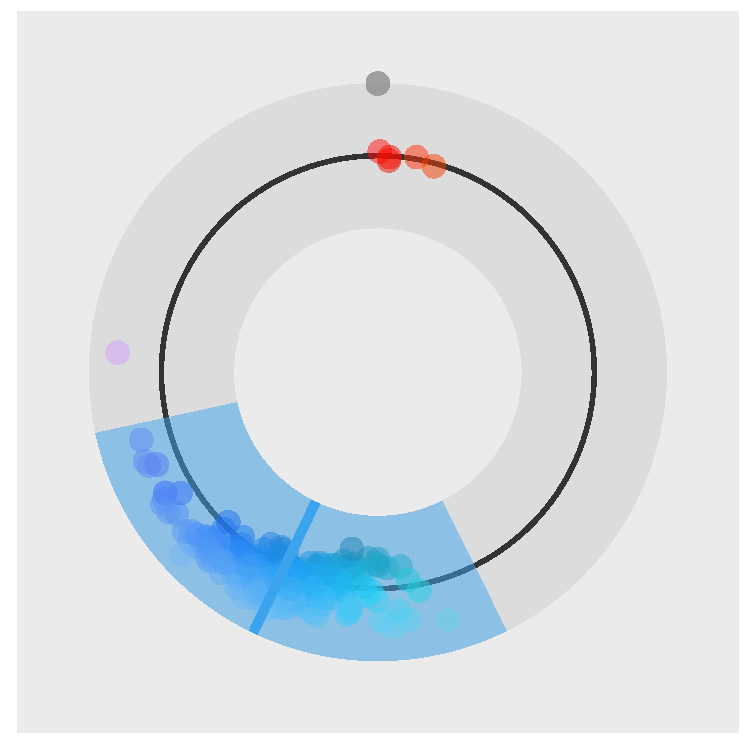
\includegraphics[width=\linewidth]{single_column.pdf}
	\caption{\textbf{A random visualization.} This is an example of a figure that spans only across one of the two columns.}
	\label{fig:column}
\end{figure}

On the other hand, \figurename~\ref{fig:whole} is an example of a figure that spans across the whole page (across both columns) of the report.

% \begin{figure*} makes the figure take up the entire width of the page
\begin{figure*}[ht]\centering 
	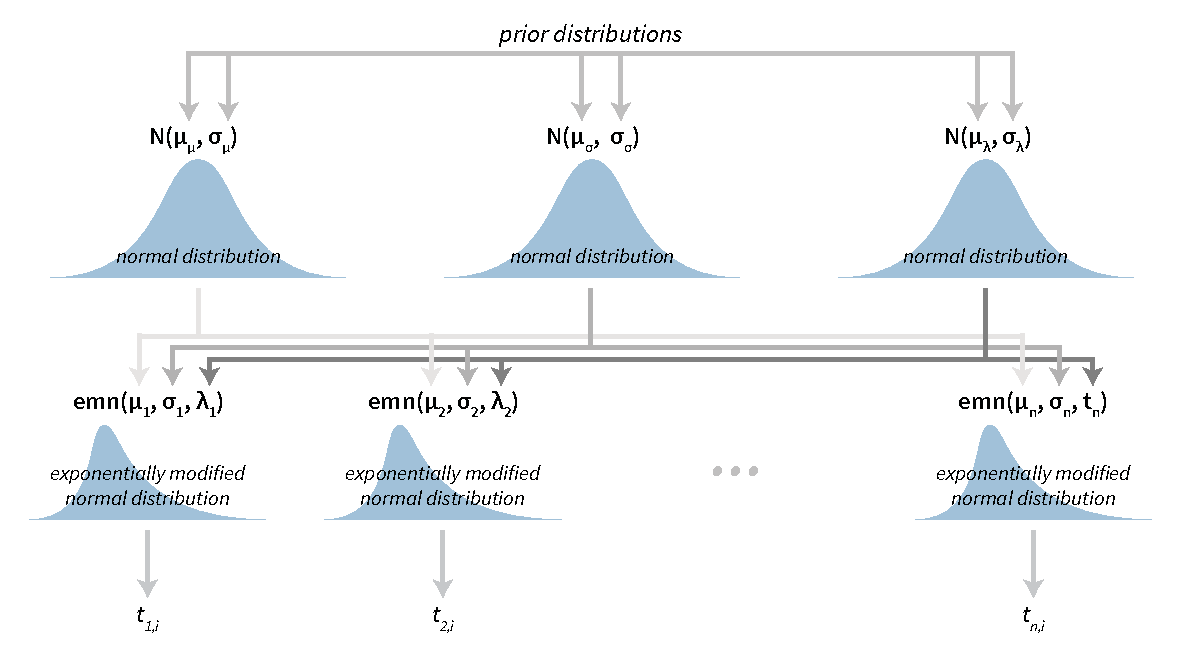
\includegraphics[width=\linewidth]{whole_page.pdf}
	\caption{\textbf{Visualization of a Bayesian hierarchical model.} This is an example of a figure that spans the whole width of the report.}
	\label{fig:whole}
\end{figure*}

\subsection*{Tables}

Use the table environment to insert tables.

\begin{table}[hbt]
	\caption{Table of grades.}
	\centering
	\begin{tabular}{l l | r}
		\toprule
		\multicolumn{2}{c}{Name} \\
		\cmidrule(r){1-2}
		First name & Last Name & Grade \\
		\midrule
		John & Doe & $7.5$ \\
		Jane & Doe & $10$ \\
		Mike & Smith & $8$ \\
		\bottomrule
	\end{tabular}
	\label{tab:label}
\end{table}

\subsection*{Code examples}

You can also insert short code examples. You can specify them manually, or insert a whole file with code. Please avoid inserting long code snippets, advisors will have access to your repositories and can take a look at your code there. If necessary, you can use this technique to insert code (or pseudo code) of short algorithms that are crucial for the understanding of the manuscript.

\lstset{language=Python}
\lstset{caption={Insert code directly from a file.}}
\lstset{label={lst:code_file}}
\lstinputlisting[language=Python]{code/example.py}

\lstset{language=R}
\lstset{caption={Write the code you want to insert.}}
\lstset{label={lst:code_direct}}
\begin{lstlisting}
import(dplyr)
import(ggplot)

ggplot(diamonds,
	   aes(x=carat, y=price, color=cut)) +
  geom_point() +
  geom_smooth()
\end{lstlisting}
\fi

%------------------------------------------------

\section*{Results}
% INSTRUCTIONS
% Use the results section to present the final results of your work. Present the results in a objective and scientific fashion. Use visualisations to convey your results in a clear and efficient manner. When comparing results between various techniques use appropriate statistical methodology.

The Table \ref{tab:evaluation} shows the success of the chosen metrics on prompt engineering and the finetuned models. For the BERTScore the mean of the F1 score is shown. $\Delta l$ shows the mean absolute difference in length of generated texts when compared to the refference texts. At this stage we used the mini testing set consisting of 232 examples.

We can see that the approach with prompt engineering generated traffic reports that were both closer to the reference reports (higher BERTScore) as well differed less in length (lower $\Delta l$). Due to the lack of BERTScore baselines for Slovenian we cannot reliably tell just how good or bad our achieved scores are, we can only compare different approaches to see which one is better. However at this point we can conclude that our current prompt engineering approach is still better.

\begin{table}[hbt]
	\caption{Achieved scores of selected metrics on the testset.}
	\centering
	\begin{tabular}{l | r r}
		\toprule
            Approach & BERTScore & $\Delta l$ \\
		\midrule
		Prompt engineering & \textbf{0.912} & \textbf{0.705}\\
		Fine Tuning GaMS 2B & 0.868 & 0.740 \\
		  Fine Tuning GaMS 9B & / & /\\
		\bottomrule
	\end{tabular}
	\label{tab:evaluation}
\end{table}

%------------------------------------------------
\iffalse
\section*{Discussion}
% INSTRUCTIONS
% Use the Discussion section to objectively evaluate your work, do not just put praise on everything you did, be critical and exposes flaws and weaknesses of your solution. You can also explain what you would do differently if you would be able to start again and what upgrades could be done on the project in the future.


%------------------------------------------------

\section*{Acknowledgments}
% INSTRUCTIONS
% Here you can thank other persons (advisors, colleagues ...) that contributed to the successful completion of your project.
\fi

%----------------------------------------------------------------------------------------
%	REFERENCE LIST
%----------------------------------------------------------------------------------------
\bibliographystyle{unsrt}
\bibliography{report}


\end{document}